\documentclass[tikz,border=8pt]{standalone}
\usepackage{xcolor}
\usetikzlibrary{arrows.meta,fit,calc,shapes.geometric}
\pgfdeclarelayer{lanes}
\pgfdeclarelayer{engine}
\pgfsetlayers{lanes,engine,main}
\newcommand{\api}[1]{{\ttfamily\detokenize{#1}}}
\definecolor{cli}{RGB}{222,235,247}
\definecolor{srv}{RGB}{253,235,215}
\definecolor{shm}{RGB}{226,240,217}
\definecolor{eng}{RGB}{255,248,225}
\definecolor{ipcbg}{RGB}{255,242,204}
\definecolor{ipccol}{RGB}{192,0,0}
\definecolor{datcol}{RGB}{56,118,29}
\tikzset{
  base/.style={draw=black!70, rounded corners=3pt, align=center,
               font=\footnotesize, inner sep=4pt, minimum height=1.0cm},
  cnode/.style={base, fill=cli},
  snode/.style={base, fill=srv},
  shmnode/.style={base, fill=shm},
  ipcnode/.style={base, fill=ipcbg, draw=ipccol!70},
  ext/.style={base, fill=black!8, draw=black!60, rounded corners=0pt},
  wnode/.style={base, fill=eng, font=\scriptsize, text width=1.4cm,
                minimum height=0.65cm, inner sep=2pt},
  note/.style={font=\scriptsize, align=center},
  flow/.style={-{Latex[length=2.5mm]}, thick, black!75},
  ipc/.style={-{Latex[length=2.5mm]}, very thick, ipccol},
  ipcb/.style={{Latex[length=2.5mm]}-{Latex[length=2.5mm]}, very thick, ipccol},
  dat/.style={-{Latex[length=2.5mm]}, thick, dashed, datcol},
  lab/.style={font=\scriptsize, inner sep=2pt},
}
\newcommand{\legend}[2]{\begin{scope}[shift={(#1,#2)}]
  \draw[flow] (0,0) -- (0.8,0) node[right, lab]{Internal flow};
  \draw[ipc]  (3.6,0) -- (4.4,0) node[right, lab]{QNX IPC (message / pulse)};
  \draw[dat]  (8.6,0) -- (9.4,0) node[right, lab]{Shared-memory access};
\end{scope}}
\begin{document}
\hyphenpenalty=10000\relax\exhyphenpenalty=10000\relax
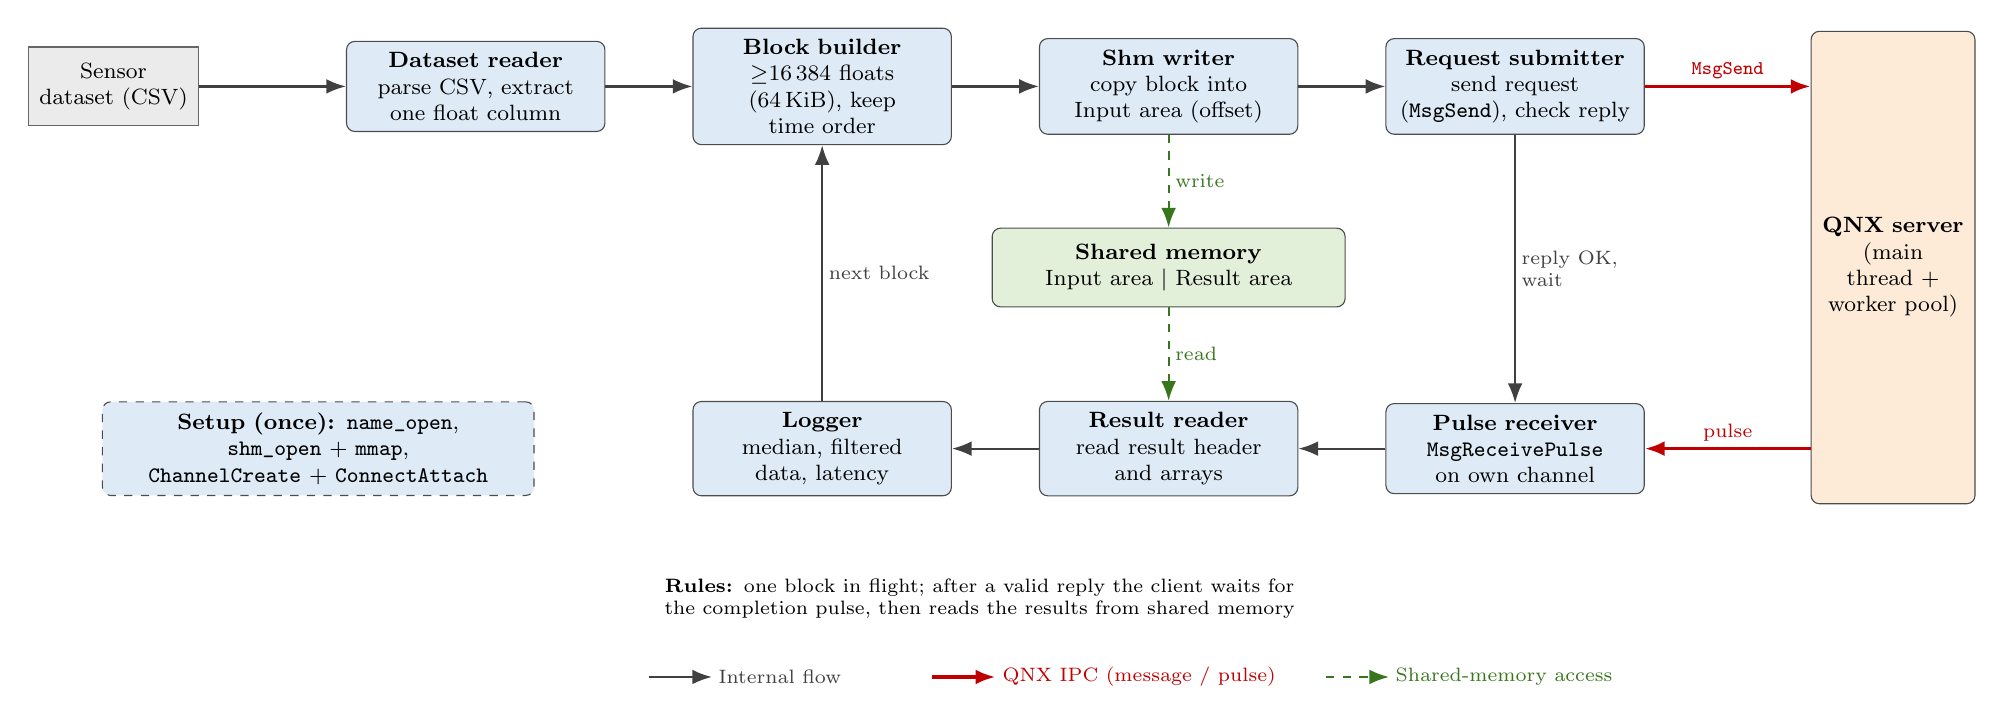
\begin{tikzpicture}
\node[ext] (ds) at (0,0) {Sensor\\ dataset (CSV)};
\node[cnode, text width=3.0cm] (r1) at (4.6,0) {\textbf{Dataset reader}\\ parse CSV, extract one float column};
\node[cnode, text width=3.0cm] (r2) at (9.0,0) {\textbf{Block builder}\\ $\geq$16\,384 floats (64\,KiB), keep time order};
\node[cnode, text width=3.0cm] (r3) at (13.4,0) {\textbf{Shm writer}\\ copy block into Input area (offset)};
\node[cnode, text width=3.0cm] (r4) at (17.8,0) {\textbf{Request submitter}\\ send request (\api{MsgSend}), check reply};
\node[shmnode, text width=4.2cm] (bar) at (13.4,-2.3) {\textbf{Shared memory}\\ Input area $|$ Result area};
\node[cnode, text width=3.0cm] (b1) at (17.8,-4.6) {\textbf{Pulse receiver}\\ \api{MsgReceivePulse} on own channel};
\node[cnode, text width=3.0cm] (b2) at (13.4,-4.6) {\textbf{Result reader}\\ read result header and arrays};
\node[cnode, text width=3.0cm] (b3) at (9.0,-4.6) {\textbf{Logger}\\ median, filtered data, latency};
\node[cnode, dashed, text width=5.2cm] (setup) at (2.6,-4.6)
  {\textbf{Setup (once):} \api{name_open}, \api{shm_open} + \api{mmap}, \api{ChannelCreate} + \api{ConnectAttach}};
\node[snode, text width=1.8cm, minimum height=6.0cm] (srv) at (22.6,-2.3) {\textbf{QNX server}\\ (main thread + worker pool)};

\draw[flow] (ds) -- (r1);
\draw[flow] (r1) -- (r2);
\draw[flow] (r2) -- (r3);
\draw[flow] (r3) -- (r4);
\draw[dat] (r3.south) -- node[right, lab]{write} (bar.north);
\draw[dat] (bar.south) -- node[right, lab]{read} (b2.north);
\draw[ipc] (r4.east) -- node[above, lab]{\api{MsgSend}} (srv.west |- r4.east);
\draw[ipc] (srv.west |- b1.east) -- node[above, lab]{pulse} (b1.east);
\draw[flow] (r4.south) -- node[right, lab, align=left]{reply OK,\\ wait} (b1.north);
\draw[flow] (b1) -- (b2);
\draw[flow] (b2) -- (b3);
\draw[flow] (b3.north) -- node[right, lab]{next block} (r2.south);

\node[note, text width=15cm] at (11.0,-6.5)
  {\textbf{Rules:} one block in flight; after a valid reply the client waits for the completion pulse, then reads the results from shared memory};
\legend{6.8}{-7.5}
\end{tikzpicture}
\end{document}